\paragraph{1.}

[25\%] Ruteo y analisis de algoritmo.

\begin{enumerate}
    \item Realice el ruteo del siguiente programa e indique que es lo que imprime. Cada vez que el valor de una variable cambie, escríbalo en una nueva fila de la tabla. Recuerde que si una variable es de tipo string, su valor debe ir entre comillas simples ’ ’.

    \textit{Importante: La tabla tiene suficientes filas}.
\begin{center}
    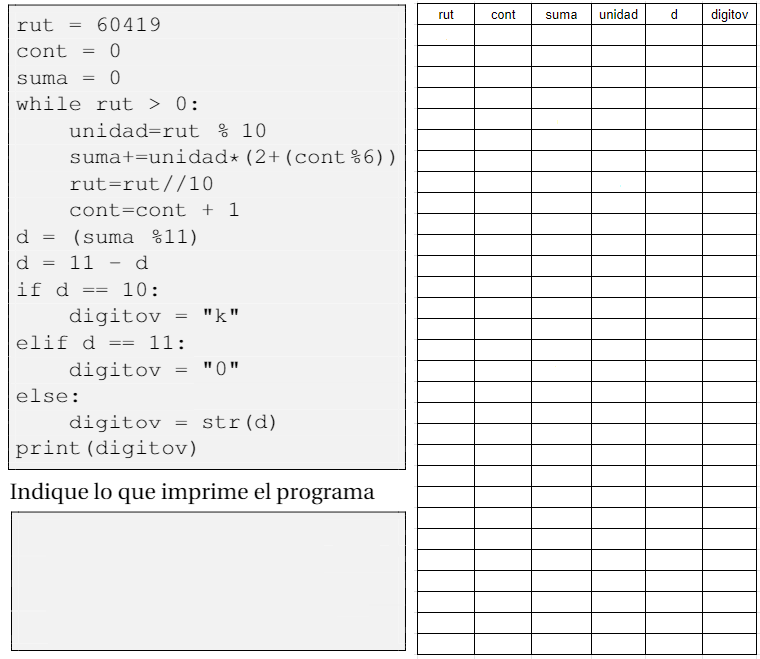
\includegraphics[scale=0.80]{Imagenes/pregunta1.png}
\end{center}

    \item Considerando el código del ruteo anterior, indique en pocas palabras que es lo que hace (o lo que usted estima que hace) dicho código.

\end{enumerate}
